\section{Introduction}

\begin{frame}
  \frametitle{High Performance Computing}
  \begin{columns}
    \column{.5\textwidth}
    \begin{center}
      \begin{figure}
        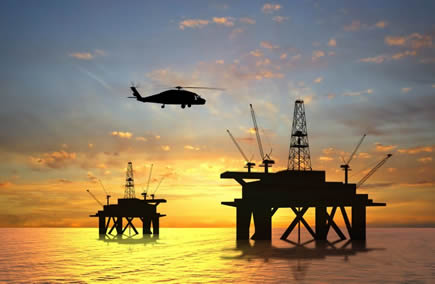
\includegraphics[scale=0.2]{figs/oil-gas-industry.jpg}\\
      \end{figure}
      \vspace{0.5cm}
      Oil and Gas
      \begin{figure}
        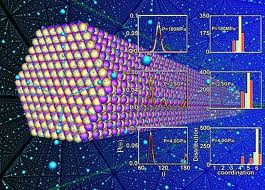
\includegraphics[scale=0.3]{figs/scientific-computing.jpg}\\
      \end{figure}
      Scientific Computing
    \end{center}
    \column{.5\textwidth}
    \begin{center}
      \begin{figure}
        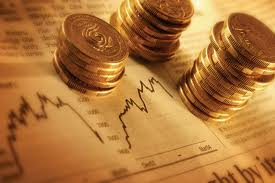
\includegraphics[scale=0.31]{figs/finance.jpg}\\
      \end{figure}
      \vspace{0.5cm}
      Finance
      \begin{figure}
        
\includegraphics[scale=0.31]{figs/ads.jpg}\\
      \end{figure}
      Online Advertising
    \end{center}
  \end{columns}
\end{frame}

\begin{frame}
  \frametitle{High Performance Computing}
  \begin{columns}
    \begin{column}{.5\textwidth}
      \begin{center}
        \begin{figure}
          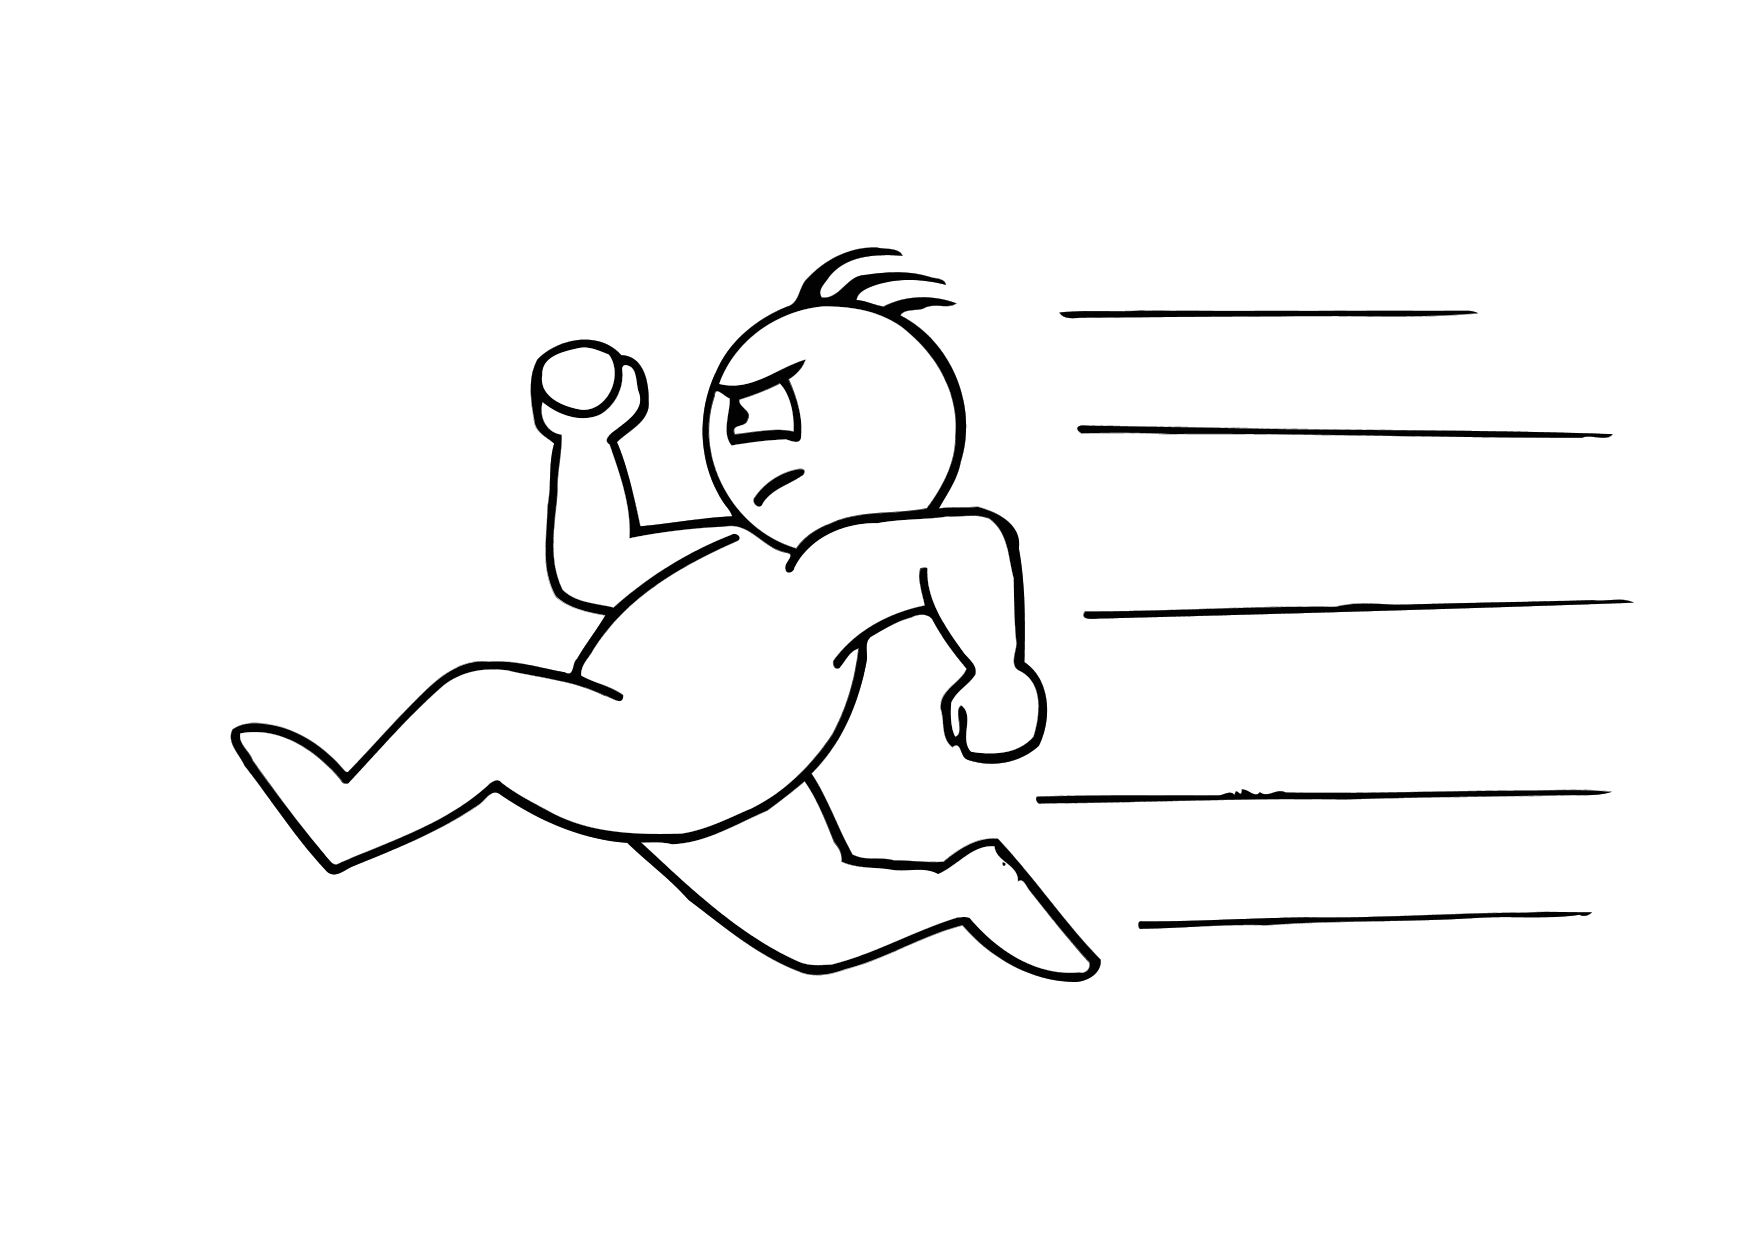
\includegraphics[scale=0.1, clip=true, trim=0 200 50 250]{figs/fast.jpg}\\
        \end{figure}
        Fast
      \end{center}
    \end{column}
    \begin{column}{.5\textwidth}
      \begin{center}
        \begin{figure}[!ht]
          \def\svgwidth{0.6\linewidth}
          \input{figs/energy-efficiency.pdf_tex}
        \end{figure}
        Energy Efficient
      \end{center}
    \end{column}
  \end{columns}
  \begin{center}
    \begin{figure}
      
\includegraphics[scale=0.3]{figs/productive.jpg}\\
    \end{figure}
    Productive
  \end{center}

\end{frame}

\begin{frame}{This Project}
  \begin{beamerboxesrounded}{Objectives}
    \begin{itemize}
    \item more efficient HPC -- using dataflow computing
    \item more productive HPC -- using aspect-oriented design
    \end{itemize}
  \end{beamerboxesrounded}
  \vspace{0.3cm}
  \begin{beamerboxesrounded}{Impact}
    \begin{itemize}
      \item first aspect-oriented compilation flow:
      \begin{itemize}
      \item for high-performance dataflow computing
      \item supporting run-time reconfiguration
      \end{itemize}
    \item 40--80\% code reduction, 4 -- 16 times less API calls
    \item produce fastest published design for Reverse Time Migration
      -- advanced seismic imaging application
    \item techniques deployed in FP7 HARNESS project
    \item best paper award candidate at ASAP 2013
    \end{itemize}
  \end{beamerboxesrounded}
\end{frame}

\begin{frame}
  \frametitle{Dataflow High-Performance Computing}
  \begin{figure}[!ht]
    \centering
    \def\svgwidth{0.9\linewidth}
    \input{figs/dataflow-both.pdf_tex}
  \end{figure}
\end{frame}

\begin{frame}
  \frametitle{CPU vs Dataflow}
  \begin{columns}
    \begin{column}{.5\linewidth}
    \vspace{-1cm}
      \begin{figure}[!ht]
        \centering
        \def\svgwidth{\linewidth}
        \input{figs/compute-cpu.pdf_tex}
      \end{figure}
      \vspace{-0.5cm}
      \begin{itemize}
      \item Fast to develop
      \item Inefficient
      \end{itemize}
    \end{column}
    \begin{column}{.5\linewidth}
    \vspace{-1cm}
      \begin{figure}[!ht]
        \centering
        \def\svgwidth{\linewidth}
        \input{figs/compute-dfe.pdf_tex}
      \end{figure}
      \vspace{-0.5cm}
      \begin{itemize}
      \item Slow to develop
      \item Efficient
      \end{itemize}
    \end{column}
  \end{columns}
\end{frame}

\begin{frame}[fragile]
  \frametitle{Kernel Optimisations Space}
  \begin{figure}[!ht]
    \centering
    \def\svgwidth{\linewidth}
    \input{figs/dfg-opt-all.pdf_tex}
  \end{figure}
\end{frame}

\begin{frame}[fragile]
  \frametitle{Issues}
  Developers must manually transform the original design to:
  \begin{enumerate}
  \item ensure I/O interface compatibility with host
  \item optimise resource usage by minimising operand width
  \item ensure result correctness by casting
  \item apply FPGA and dataflow specific optimisations
  \item replicate computational pipelines
  \end{enumerate}
\vspace{0.5cm}
  \begin{beamerboxesrounded}{The Problem}
    Mixing optimisations with functional code makes it:
    \begin{itemize}
    \item harder to infer optimal designs (more constraints)
    \item harder to automate design space exploration
    \item impossible to re-target optimisations automatically
    \end{itemize}
  \end{beamerboxesrounded}
\end{frame}
